\documentclass[12pt,a4paper]{article}
\usepackage[italian]{babel}
\usepackage[T1]{fontenc}
\usepackage[latin1]{inputenc}
\usepackage{graphicx}
\usepackage{amsmath}
\usepackage{subfig}
\date{}
\begin{document}
\title{Strutture Aeronautiche\\ Esercitazione 1 \\ Prof.re Franco Mastroddi}
\author{Matteo Hakimi 1455230}
\maketitle
\begin{figure}[htbp]
\centering

\includegraphics[width=100mm]{Immagini/sapienzalogo}
\end{figure}
\newpage
\tableofcontents
\newpage

\section{Introduzione}
Si vuole calcolare il campo di spostamenti,in diverse condizioni di carico di una struttura costituita da un cassone alare incastrato da un lato ,in lega metallica
leggera (Alluminio E=68GPa  $\nu =0.3$  $\rho=2650\frac{Kg}{m^3}$ ) di lunghezza longitudinale pari a L=4m , una cross section rettangolare di dimensioni 0.6mx0.1m
costituita da 4 pannelli di spessore t=0.003m , e da 4 irriggidimenti ( longheroni) posti ai vertici della sezione trasversale, che percorrono la struttura nella direzione longitudinale, di sezione pari a $ A=0.0025{m^2} $  .\\
Il calcolo verr\'a svolto tramite l'uso di solutore agli elementi finiti, discretizzando opportunamente la struttura.
Infine si effettuer\'a il confronto della soluzione con quella ottenuta per via analitica.
 
\begin{figure}[htbp]
\centering
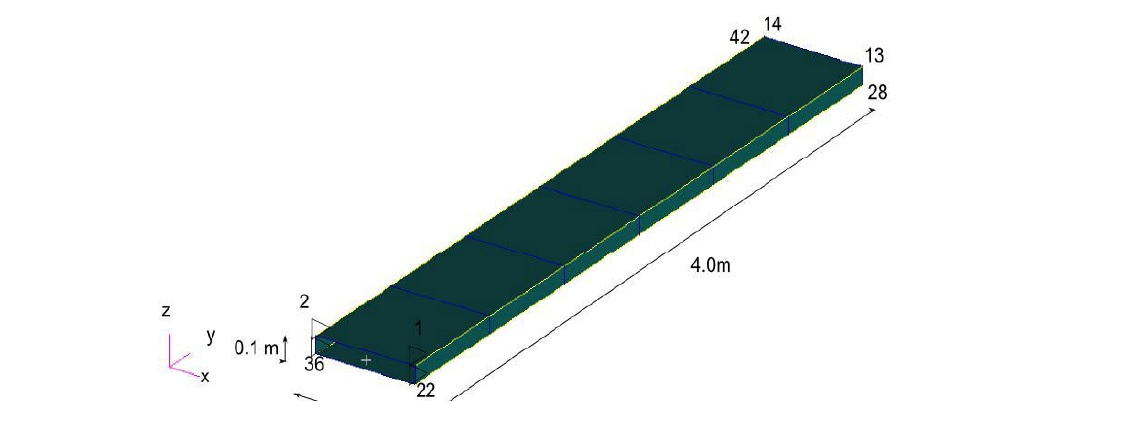
\includegraphics[width=150mm]{Immagini/Cassone}
\caption{Cassone Alare}
\end{figure}

\section{Carico applicato lungo z}
Il primo caso che verr\'a analizzato \'e il calcolo della risposta statica (SOL 101) della struttura sottoposta ad un carico di estremit\'a P=10000N realizzato con la ripartizione
su due forze concentrate applicate a due nodi dell'estremit\'a alare (ciascuna di intensit\'a di 5000N ) uno al
bordo d'attacco a l'altro al bordo d'uscita (nodi 28 e 42) entrambe in direzione verticale verso l'alto. Successivamente verranno rimossi i logheroni e verr\'a reiterato il calcolo.
Il modello agli elementi finiti \'e costituito da elementi monodimensionali (ROD con sezione pari a $ 0.0025 m^2 $ )
ed elementi bidimensionali (SHELL con spessore di 0.003 m).

\subsection{Soluzione con irridimenti longitudinali}
Si \'e rappresentata la deformata,attraverso l'ausilio di Matlab, lungo una linea di nodi di un bordo di uno dei
longheroni,dove si riportano gli spostamenti lungo z al variare dell'ascissa y adimensionalizzata rispetto alla
lunghezza longitudinale del cassone,a confronto con i risultati offerti dalla teoria della trave inflessa.
\begin{figure}[htbp]
\centering
\includegraphics[width=150mm]{Immagini/Confrontoanalitico}
\caption{Confronto soluzione analitica con Fem caso flessione}
\end{figure}
\newpage
Si pu\'o notare come la soluzione ottenuta col solutore presenta un andamento molto prossimo a
quello offerto dalla teoria analitica (trave Eulero Bernulli).
Si riporta nel dettaglio il valore di displacement e rotazione del nodo 13
\begin{center}
\begin{tabular}{c c c c}
\hline
Point ID & T1 & T2  &  T3\\
13 & 3.666635E-06 & -1.700912E-03 & 9.253278E-02\\
\hline
Point ID & R1  &  R2  &  R3\\
13 & 3.407605E-02 & 5.869038E-05 & 4.054110E-05\\
\hline
\end{tabular}
\end{center}
L' errore relativo al tip sullo spostamento lungo z \'e pari a $ \epsilon =$ 3.99 $10^{-3} m$  rispetto a quello analitico (9.6530920 $10^{-2} m$) e sulla rotazione attorno a x di $\epsilon =$2.12$10^{-3} rad$ rispetto a quello analitico (3.6199095  $10^{-2}$ rad).
Si riportano i valori delle componenti della reazione vincolare del nodo 1:
\begin{center}
\begin{tabular}{c c c c}
\hline
Point ID& T1 & T2 & T3\\
1 & -9.921290E+03 & 1.999500E+05 & -2.498879E+03\\
\hline
Point ID & R1 & R2 & R3\\
1 & -2.497716E+00 &-1.682029E-01 & 2.796296E+00\\
\hline
\end{tabular}\\ 
\end{center}
La forza lungo \l'asse z \'e quella necessaria per contrastare il carico applicato (un quarto, essendo 4 i nodi
vincolati). La forza lungo l'asse y \'e positiva essendo il nodo 1 sulla parte superiore del cassone infatti \'e
necessaria per contrastare la compressione indotta sulla parte superiore dalla flessione. Sui due nodi vincolati
della parte inferiore sono presenti reazioni vincolari uguali e contrarie per contrastare la trazione. La somma
delle 4 reazioni vincolari lungo y \'e nulla. Il momento attorno a x generato dalle forze delle reazioni vincolari
agenti lungo y equilibra il momento flettente generato dal carico.

\subsection{Soluzione senza irrigidimenti longitudinali}
Analogamente a quanto visto nel primo sottocaso si procede con il calcolo con l'unica eccezione che questa volta sono stati rimossi i longheroni
(Rod). Nel codice corrisponde a porre uguale a 0 l'area dei correnti.\\
Si \'e notata una notevole differenza nella soluzione a dimostrazione del fatto che i correnti, contribuiscono a contrastare la deformazione del
cassone quando \'e applicato un carico lungo l'asse z all'estremit\'a del cassone. Sempre nel nodo 13 si ottiene:\\
\begin{center}
\begin{tabular}{c c c c}
\hline
Point ID& T1 & T2 & T3\\
13 & 1.255903E-05 & -6.139704E-03 & 3.264377E-01\\
\hline
Point ID & R1 & R2 & R3\\
13 & 1.227434E-01 & 2.282389E-04 & 1.419131E-04\\
\hline
\end{tabular}\\ 
\end{center}
Si riporta inoltre il confronto lungo una linea di nodi disposti lungo un longherone tra  il primo sottocaso e il secondo.\\
\begin{figure}[htbp]
\centering
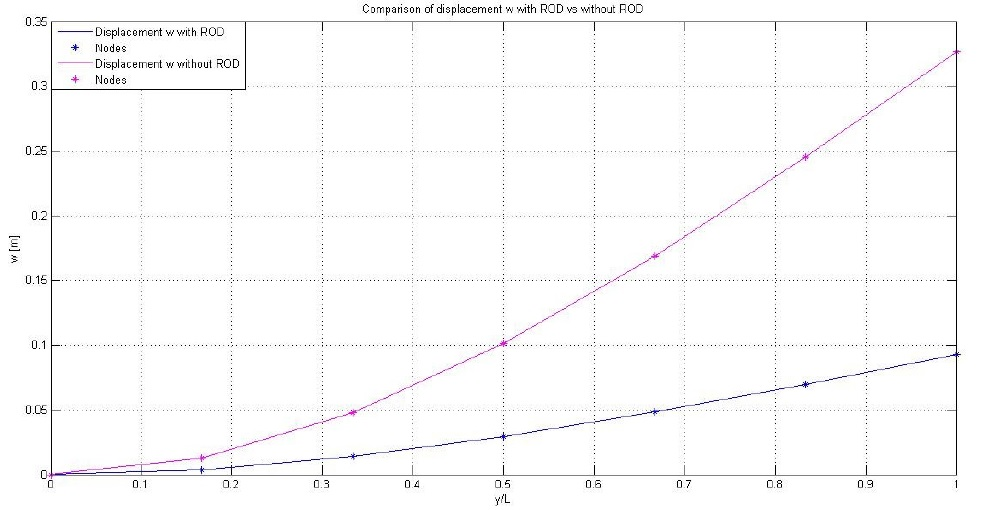
\includegraphics[width=150mm]{Immagini/confrontorod}
\caption{Confronto spostamenti flessionali con irrigidimenti e senza}
\end{figure}\\

\section{Carico applicato lungo x}
Il secondo caso fa riferimento alla stessa geometria e carico del primo caso differendo da quest'ultimo per la direzione di applicazione del carico stesso; infatti il carico \'e stato ripartito sui nodi 13 e 28 e la sua direzione \'e parallela
all'asse x.\\
Ora si nota che la deformazione pi\'u consistente si ha lungo l'asse x e che essa \'e minore della massima deformazione lungo l'asse z trovata nel caso 1 siccome l'inerzia della sezione attorno l'asse z \'e 1.062 $10^{-3} {m^4}$,
 maggiore rispetto a quella attorno l'asse x (3.45 $10^{-5} {m^4}$):\\
 \begin{center}
 \begin{tabular}{c c c c}
 \hline
 Point ID& T1 & T2 & T3\\
 13 & 3.371049E-03 & -3.328972E-04 & -3.680786E-07\\
 \hline
 Point ID & R1 & R2 & R3\\
 13 & -2.064145E-06 & -3.728811E-07 & -1.167187E-03\\
 \hline
 \end{tabular}\\ 
 \end{center}
Lo spostamento al tip differisce del $\epsilon=$4.11 $10^{-4} m$ da quello analitico offerto dalla teoria della trave ( 2.9596744 $10^{-3} m$). La rotazione al tip calcolata con MSC Nastran \'e di -1.167187 $10^{-3} rad$ mentre quella calcolata con la
teoria della trave \'e -1.1098779 $10^{-3} rad$ .

\section{Momento torcente applicato attorno a y}
Nel terzo caso sono state applicate due forze, di intensit\'a pari a 5000 N all'estremit\'a del cassone. Una verso l'alto sul nodo 28 e
una verso il basso sul nodo 14. Complessivamente ne deriva un momento torcente applicato di intensit\'a pari a  3000 Nm, dato il braccio b=0.6 m.Analogamente a quanto visto nella prima sezione il calcolo della risposta statica verr\'a reiterato successivamente avendo rimosso gli irrigidimenti longitudinali.

\subsection{Soluzione con irrigidimenti longitudinali}
 In figura \'e riportato il confronto tra la soluzione del modello approssimato e
quella analitica ottenuta con la teoria di Bredt, e il campo di spostamenti e rotazioni per il nodo 13.
\begin{figure}[htbp]
\centering
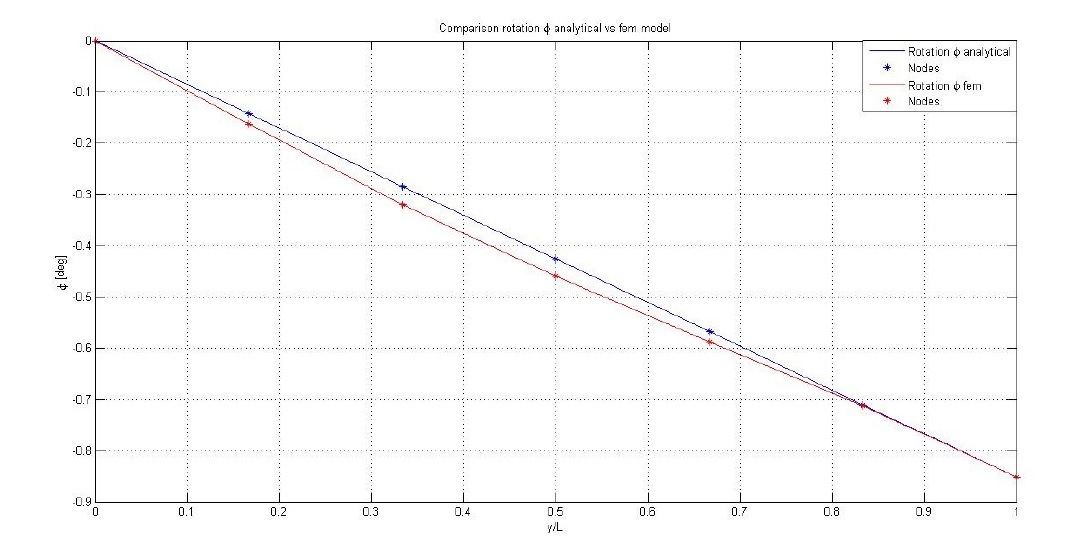
\includegraphics[width=150mm]{Immagini/confrontoanaliticotorsione}
\caption{Confronto soluzione analitica con Fem caso torsione}
\end{figure}
\newpage
Per il nodo 13 si ha:\\
 \begin{center}
 \begin{tabular}{c c c c}
 \hline
 Point ID& T1 & T2 & T3\\
 13 & 7.160255E-04 & 5.416122E-05 & -4.391133E-03\\
 \hline
 Point ID & R1 & R2 & R3\\
 13 & -1.214607E-03 & 1.486716E-02 & 1.097381E-04\\
 \hline
 \end{tabular}\\ 
 \end{center}
Sono stati analizzati i risultati e confrontati con quelli analitici forniti dalla teoria di Bredt (G=26.9 GPa,
$S=0.06 m^2  B=8.31$ $10^5 Nm^2$). La rotazione in funzione di y fornita dalla teoria di Bredt risulta essere:
$\phi(y)=$3.61 $10^{-3}$y . La rotazione massima risulta essere quindi di 1.444 $10^{-2} rad$, in buon accordo con i risultati
di Nastran (1.486716 $10^{-2} rad$). L'errore \'e pari a $\epsilon=$  4.27 $10^{-4} rad$.

\subsection{Soluzione senza irrigidimenti longitudinali}
 Si procede con il calcolo della soluzione rimuovendo gli irrigidimenti .In figura viene riportato il confronto tra il caso attuale e
quello precedente
\begin{figure}[htbp]
	\centering
	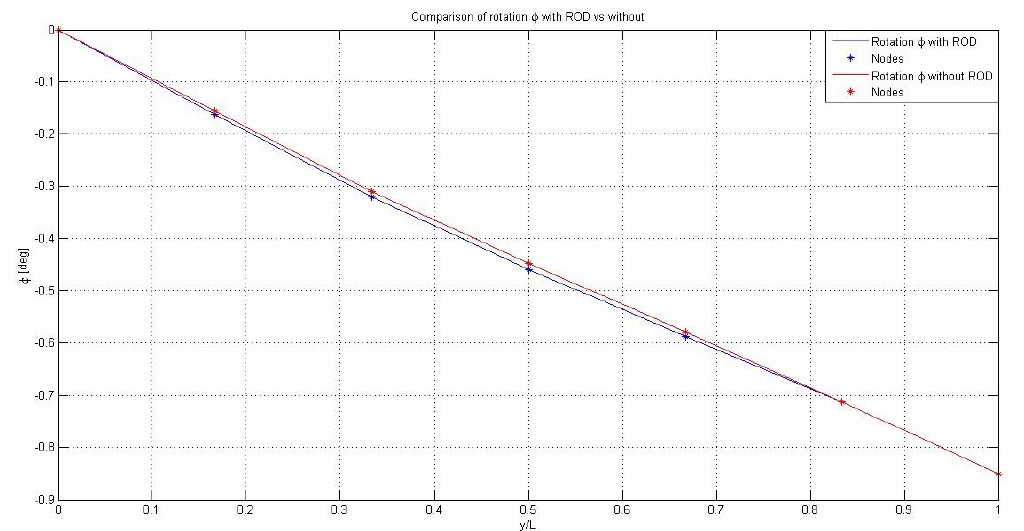
\includegraphics[width=150mm]{Immagini/confrontorodtors}
	\caption{Confronto rotazione torsionale con irrigidimenti e senza}
\end{figure}
\newpage
Si pu\'o osservare che nel caso della torsione pura i longheroni non influenzano in modo
significativo il comportamento a torsione della struttura.
A titolo esplicativo vengono, infine, riportati gli spostamenti e rotazioni del nodo 13.\\
 \begin{center}
 \begin{tabular}{c c c c}
 \hline
 Point ID& T1 & T2 & T3\\
 13 & 7.303965E-04 & 4.580828E-05 & -4.479178E-03\\
 \hline
 Point ID & R1 & R2 & R3\\
 13 & -1.048825E-03 & 1.487031E-02 & 8.150756E-05\\
 \hline
 \end{tabular}\\ 
 \end{center}

\end{document}